In a similar manner, the chart below shows evolution of BMI of issues by quarter, allowing us to check how issues are being resolved by the community in the last quarter compared to previous ones.

\begin{tabular}{p{9cm} p{5cm}}
	\vspace{0pt} 
	\hspace*{-6cm}  
	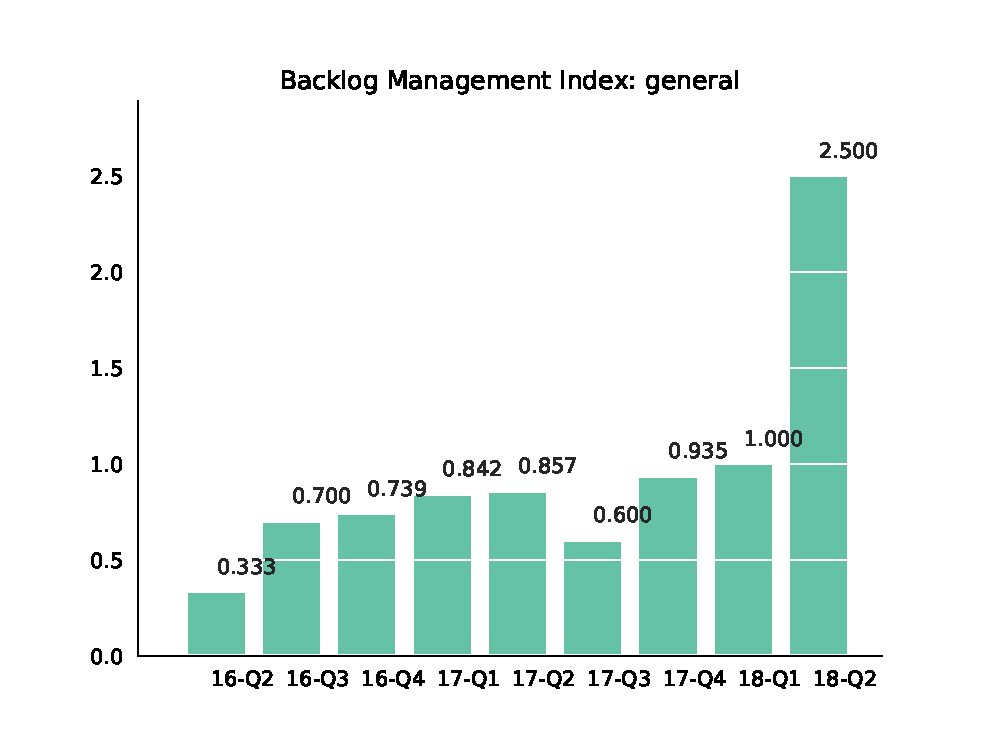
\includegraphics[scale=.75]{process/github_issues_bmi_tickets.eps}
	& 
	\vspace{0pt}
	\begin{tabular}{l|l}%
		\bfseries Period & \bfseries Closed/Subm. % specify table head
		\csvreader[head to column names]{process/github_issues_bmi_tickets.csv}{}% use head of csv as column names
		{\\\Date  & \bmi}
	\end{tabular}
\end{tabular}

Besides, the next chart deals with timing. It shows the mean and median times to merge pull requests in GitHub (TTM, defined in section \ref{overview})--in days--for last quarter compared to previous ones.


\begin{tabular}{p{9cm} p{5cm}}
	\vspace{0pt} 
	\hspace*{-6cm}  
	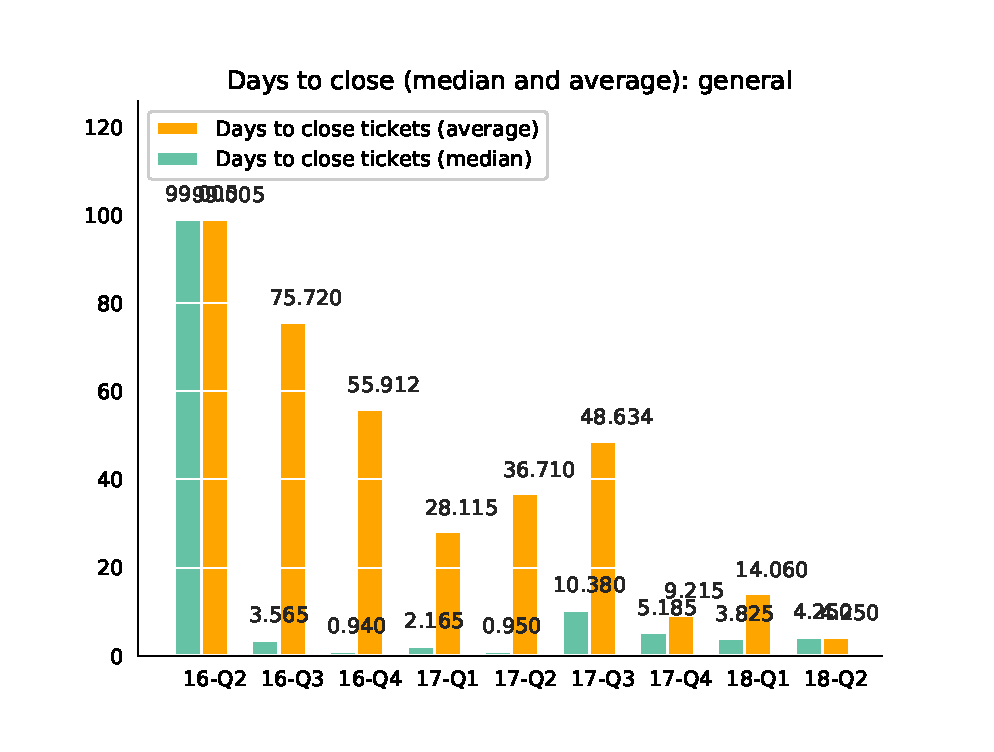
\includegraphics[scale=.75]{process/github_issues_days_to_close_ticket_average_github_issues_days_to_close_ticket_median.eps}
	& 
	\vspace{0pt}
	\begin{tabular}{l|r|r|}%
		\bfseries Period & \bfseries Median & \bfseries Mean % specify table head
		\csvreader[head to column names]{process/github_issues_days_to_close_ticket_average_github_issues_days_to_close_ticket_median.csv}{}% use head of csv as column names
		{\\\Date & \daystocloseticketmedian & \daystocloseticketaverage}
	\end{tabular}
\end{tabular}